\documentclass[dutch]{ucll-slides}
\usepackage{pxfonts}
\usepackage{tikz}
\usepackage{calc}
\usepackage{ucll-code}
\usepackage{hyperref}


\usetikzlibrary{calc,shadows,tikzmark,math,shadings}

\coursename{Scripttalen}
\title{Python}



\begin{document}

\maketitle

\section{Waarom Python?}

\subsection{Wie Gebruikt Python?}

\frame{\tableofcontents[currentsubsection]}


\begin{frame}
  \frametitle{Rankings}
  \begin{columns}
    \column{5cm}
    \begin{center}
      \begin{tabular}{cc}
        \textbf{Ranking} & \textbf{Taal} \\
        \toprule
        1 & Java \\
        2 & C \\
        3 & C++ \\
        4 & C$^\sharp$ \\
        5 & Python \\
      \end{tabular}
      \vskip5mm
      \link{http://www.tiobe.com/tiobe-index/}{\tiny TIOBE Index for January 2017}
    \end{center}
    \column{5cm}
    \begin{center}
      \begin{tabular}{cc}
        \textbf{Ranking} & \textbf{Taal} \\
        \toprule
        1 & JavaScript \\
        2 & Java \\
        3 & Python \\
        4 & CSS \\
        5 & PHP \\
      \end{tabular}
      \vskip5mm
      \link{http://githut.info/}{\tiny githut.info}
    \end{center}
  \end{columns}
  \vskip5mm
  \begin{quote}
    Eight out of the top 10 universities now use Python to introduce programming --- \link{http://www.javaworld.com/article/2452940/learn-java/python-bumps-off-java-as-top-learning-language.html}{Javaworld}
  \end{quote}
\end{frame}


\begin{frame}
  \frametitle{Gebruik}
  \begin{center}
    \begin{tikzpicture}
      \node at (2, 3) {
\includegraphics[width=2cm]{google.png}};
      \node at (-2, 0) {
\includegraphics[width=3cm]{dropbox.png}};
      \node at (4, -1) {
\includegraphics[width=1cm]{facebook.png}};
      \node at (-1, 2) {
\includegraphics[width=2cm]{quora.png}};
      \node at (3, 1) {
\includegraphics[width=3cm]{reddit.png}};
      \node at (-2, -2) {
\includegraphics[width=2cm]{pinterest.png}};
      \node at (1, -2) {
\includegraphics[width=2cm]{youtube.png}};
    \end{tikzpicture}
  \end{center}
\end{frame}

\subsection{Eenvoud}

\frame{\tableofcontents[currentsubsection]}

\begin{frame}
  \frametitle{Hello World!}
  \begin{itemize}
    \item Traditie gebiedt dat het eerste programma dat je schrijft
          in een nieuwe taal ``Hello World'' is
    \item Dit programma moet ``Hello World'' afprinten
  \end{itemize}
\end{frame}

\begin{frame}
  \frametitle{Java}
  \code[language=java,font=\small,width=.9\linewidth]{hello-world.java}
  \begin{tikzpicture}[overlay,remember picture,
                      message/.style={opacity=0.75,text opacity=1.0,drop shadow,fill=blue!50,font=\small},
                      link/.style={-latex}]

    \onslide<2->{
      \codeoverlinex{class}
      \node[message] (message) at ($ (class) + (0,1) $) {Klassedeclaratie};
      \draw[link] (message) -- (class);
    }
    \onslide<3->{
      \codeoverlinex{public}
      \node[message] (message) at ($ (public) + (-1,1) $) {Access modifier};
      \draw[link] (message) -- (public);
    }
    \onslide<4->{
      \codeoverlinex{static}
      \node[message] (message) at ($ (static) + (1,1) $) {Klassemethodes};
      \draw[link] (message) -- (static);
    }
    \onslide<5->{
      \codeoverlinex{void}
      \node[message] (message) at ($ (void) + (1,2) $) {Returntypes};
      \draw[link] (message) -- (void);
    }
    \onslide<6->{
      \codeoverlinex{main}
      \node[message] (message) at ($ (main) + (1.5,1) $) {Entry point};
      \draw[link] (message) -- (main);
    }
    \onslide<7->{
      \codeoverlinex{array}
      \node[message] (message) at ($ (array) + (2,2) $) {Parametertypes, arrays};
      \draw[link] (message) -- (array);
    }
    \onslide<8->{
      \codeunderlinex{println}
      \node[message] (message) at ($ (println) + (0,-1) $) {Member access (onzuiver wegens static), methodeoproep};
      \draw[link] (message) -- (println);
    }
    \onslide<9->{
      \codeunderlinex{string}
      \node[message] (message) at ($ (string) + (0,-2) $) {String literals};
      \draw[link] (message) -- (string);
    } 
    \onslide<10->{
      \codeoverlinex{semicolon}
      \node[message] (message) at ($ (semicolon) + (0,1) $) {Random syntax};
      \draw[link] (message) -- (semicolon);
    } 
 \end{tikzpicture}
\end{frame}

\begin{frame}
  \frametitle{Python}
  \code[language=python,font=\small,width=.4\linewidth]{hello-world.py}
  \begin{tikzpicture}[overlay,remember picture,
                      message/.style={opacity=0.75,text opacity=1.0,drop shadow,fill=blue!50,font=\small},
                      link/.style={-latex}]

    \onslide<2->{
      \codeoverlinex{py print}
      \node[message] (message) at ($ (py print) + (0,1) $) {Functies};
      \draw[link] (message) -- (py print);
    }
    \onslide<3->{
      \codeunderlinex{py string}
      \node[message] (message) at ($ (py string) + (0,-1) $) {String literals};
      \draw[link] (message) -- (py string);
    }
 \end{tikzpicture}
\end{frame}

\begin{frame}
  \frametitle{Eenvoud}
  \begin{itemize}
    \item Python is ``gelaagder''
    \item Enkel gebruiken wat je nodig hebt
    \item Nieuwe concepten komen geleidelijk aan bod
    \item Kleine initi\"ele leerdrempel
  \end{itemize}
\end{frame}

\subsection{REPL}

\frame{\tableofcontents[currentsubsection]}

\begin{frame}
  \frametitle{REPL}
  \begin{center}
    \begin{tabular}{l}
      \textbf{R}ead \\
      \textbf{E}val \\
      \textbf{P}rint \\
      \textbf{L}oop
    \end{tabular}
  \end{center}
  \begin{itemize}
    \item Laat interactief programmeren toe
    \item Gemakkelijk om code uit te testen
    \item Geen \texttt{main} methode nodig met sysouts
  \end{itemize}
\end{frame}


\subsection{Toepassingen}

\frame{\tableofcontents[currentsubsection]}

\begin{frame}
  \frametitle{Toepassingen: Java}
  \begin{itemize}
    \item Elke taal heeft zijn specialiteit en doelbpubliel
    \item Java bedoeld voor ``programming in the large''
          \begin{itemize}
            \item Grote teams
            \item 100k+ lijnen code
          \end{itemize}
    \item Statische typering als contracten tussen teamleden
          \begin{itemize}
            \item Als u mij 2 integers geeft, beloof ik u een double terug, tenzij ik u een
                  \texttt{WrongIntegerException} toewerp
          \end{itemize}
    \item Klassen om voor structuur te zorgen
    \item Relatief weinig taalfeatures om kloof tussen goede en slechte programmeurs te vermijden
    \item Heeft veel weg van logge bureaucratie
  \end{itemize}
\end{frame}

\begin{frame}
  \frametitle{Toepassingen: Python}
  \begin{itemize}
    \item Python is ``lean and mean''
    \item Code doorgaans korter dan equivalente Javacode
    \item Python goed voor kleine en middelgrote projecten
          \begin{itemize}
            \item Wegwerpprogramma's
            \item Automatisatie simpele taken
            \item Ondersteunende software (bv.~leveleditor voor spel)
          \end{itemize}
    \item Python als scripting taal
          \begin{itemize}
            \item Plugins voor grote apps in Python
            \item Bv.~Gimp, Inkscape
          \end{itemize}
    \item Python niet aangeraden voor grote projecten
          \begin{itemize}
            \item Te weinig taalondersteuning
          \end{itemize}
  \end{itemize}
\end{frame}



%%% Local Variables:
%%% mode: latex
%%% TeX-master: "python"
%%% End:

\section{Compilatie vs Interpretatie}

\frame{\tableofcontents[currentsection]}

\begin{frame}
  \frametitle{Taal van de CPU}
  \begin{center}
    
\includegraphics[width=5cm]{cpu.jpg}
  \end{center}
  \begin{itemize}
    \item CPU begrijpt enkel machinecode
    \item CPU kan instructies in machinecode razendsnel uitvoeren
    \item Hel voor de mens om in te programmeren
  \end{itemize}
\end{frame}

\begin{frame}
  \frametitle{Programmeertalen}
  \begin{itemize}
    \item Talen ontwikkeld om het de mens gemakkelijker te maken
    \item Bv.~oudste taal: FORTRAN (Formula Translator)
  \end{itemize}
  \begin{center}
    \begin{tikzpicture}[code/.style={draw,drop shadow,fill=white}]
      \node[code,font=\small] (asm) at (0,0) {
        \parbox{6cm}{
          \code[width=\linewidth,frame=none]{addition.asm}
        }
      };
      \node[anchor=west,code,font=\small] (cpp) at ($ (asm.east) + (1,0) $) {
        \ttfamily\small z = x + y
      };
      \draw[-latex] (asm.east) -- (cpp.west);
    \end{tikzpicture}
  \end{center}
\end{frame}

\begin{frame}
  \frametitle{Vertaling}
  \begin{itemize}
    \item Programmeertaal moet vertaald worden naar machinecode
    \item Spectrum aan verschillende technieken mogelijk
    \item Uiteindes: compilatie en interpretatie
  \end{itemize}
  \begin{center}
    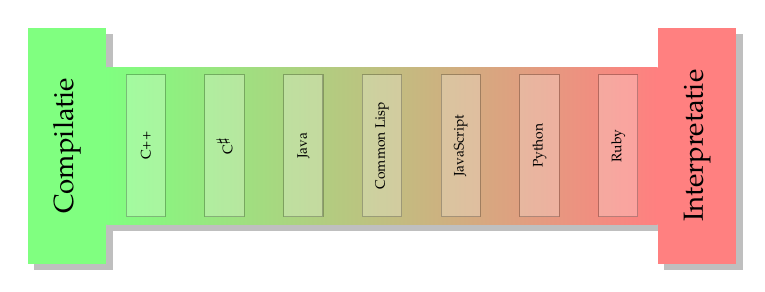
\begin{tikzpicture}[approach/.style={drop shadow,rotate=90,minimum width=3cm,minimum height=1cm},
                        language/.style={font=\tiny,minimum width=1.8cm,minimum height=.5cm,rotate=90,opacity=0.25,draw,text opacity=1,fill=white}]
      \node[approach,fill=green!50] (compilation) at (-4,0) {Compilatie};
      \path[left color=green!50,right color=red!50,drop shadow] (-3.5,-1) rectangle (3.5,1);
      \node[approach,fill=red!50] (interpretation) at (4,0) {Interpretatie};
      \node[language] (cpp) at (-3,0) {C++};
      \node[language] (python) at (2,0) {Python};
      \node[language] (ruby) at (3,0) {Ruby};
      \node[language] (java) at (-1,0) {Java};
      \node[language] (csharp) at (-2,0) {C$^\sharp$};
      \node[language] (javascript) at (1,0) {JavaScript};
      \node[language] (lisp) at (0,0) {Common Lisp};
    \end{tikzpicture}
  \end{center}
\end{frame}

\subsection{Compilatie}

\frame{\tableofcontents[currentsubsection]}

\begin{frame}
  \frametitle{Compilatie: Analogie}
  \begin{itemize}
    \item Je spreekt enkel Nederlands
    \item Je krijgt een keukenrecept
    \item Oorspronkelijk was het recept in het Japans
    \item Gelukkig werd het op voorhand vertaald
    \item Je kan er dus effici\"ent mee overweg
  \end{itemize}
\end{frame}

\begin{frame}
  \frametitle{Compilatie}
  \structure{Voordelen}
  \begin{itemize}
    \item Code wordt effici\"ent uitgevoerd
    \item Compilatie checkt op fouten
  \end{itemize}
  \vskip5mm
  \structure{Nadelen}
  \begin{itemize}
    \item Alle code moet op voorhand beschikbaar zijn
    \item Code genereren at runtime gaat niet
    \item Code kan niet aangepast worden tijdens uitvoering
    \item Hercompilatie nodig bij wijziging code
  \end{itemize}
\end{frame}

\subsection{Interpretatie}

\frame{\tableofcontents[currentsubsection]}

\begin{frame}
  \frametitle{Compilatie: Analogie}
  \begin{itemize}
    \item Je spreekt enkel Nederlands
    \item Je krijgt een keukenrecept
    \item Het recept is in het Japans
    \item Je krijgt een woordenboek en grammaticaboek
    \item 't Koken gaat wat minder effici\"ent gebeuren
  \end{itemize}
\end{frame}

\begin{frame}
  \frametitle{Interpretatie}
  \structure{Voordelen}
  \begin{itemize}
    \item Nieuwe code kan tijdens uitvoering geproduceerd worden
    \item Code kan aangepast worden tijdens uitvoering
    \item Meer flexibiliteit in het algemeen
  \end{itemize}
  \vskip5mm
  \structure{Nadelen}
  \begin{itemize}
    \item Code kan nog allerhande typfouten bevatten die pas tijdens uitvoering worden opgemerkt
    \item Code werkt veel trager omdat het ter plekke nog vertaald moet worden
  \end{itemize}
\end{frame}



%%% Local Variables:
%%% mode: latex
%%% TeX-master: "python"
%%% End:

\section{Types}

\frame{\tableofcontents[currentsection]}

\begin{frame}
  \frametitle{Op CPU Niveau}
  \begin{center} \ttfamily
    10010101 11001111 11000110 00010110 \\
    10110110 10010101 11000101 11010110 \\
    01100011 10110101 00101011 00101011 \\
    10010101 10111010 01000011 10101111 \\
    01011101 00110110 11101111 01010110 \\
    10111010 01010010 11001010 10110101 \\
    10010101 10100111 01010011 01110100 \\
    01110111 01101010 10110101 01011110 \\
  \end{center}
  \begin{itemize}
    \item Wat stellen deze bits voor?
  \end{itemize}
\end{frame}

\begin{frame}
  \frametitle{Interpretatie van Bits}
  \begin{itemize}
    \item Neem een png bestand
    \item Verander de extensie naar mp3
          \begin{itemize}
            \item Wat gebeurt er bij het afspelen ervan?
          \end{itemize}
    \item Verander de extensie naar txt
          \begin{itemize}
            \item Wat toont notepad?
          \end{itemize}
    \item Verander de extensie naar zip
          \begin{itemize}
            \item Welke bestanden steken erin?
          \end{itemize}
    \item Extensie geeft informatie over inhoud bestand
          \begin{itemize}
            \item Geeft betekenis aan bits
          \end{itemize}
  \end{itemize}
\end{frame}

\begin{frame}
  \frametitle{Types in Assembly}
  \begin{itemize}
    \item Assembly kent geen types
    \item Alles zijn bits
  \end{itemize}
  \code[language=java,font=\small,extra keywords={bits},title=Als Java Assembly was]{bits.java}
\end{frame}

\begin{frame}
  \frametitle{Typefouten}
  \begin{itemize}
    \item Programmeertalen willen extra ondersteuning bieden
    \item Willen betekenis (= type) toekennen aan bits
          \begin{itemize}
            \item Deze bits vormen een integer
            \item Deze bits vormen een kleur
            \item \dots
          \end{itemize}
    \item Toegelaten operaties hangt af van type
          \begin{itemize}
            \item Men kan een tv niet laten remmen
            \item Men kan een auto niet van zender veranderen
          \end{itemize}
    \item Taal checkt dat operaties enkel uitgevoerd worden op objecten met juist type
  \end{itemize}
\end{frame}

\begin{frame}
  \frametitle{Typesystemen}
  \begin{center}
    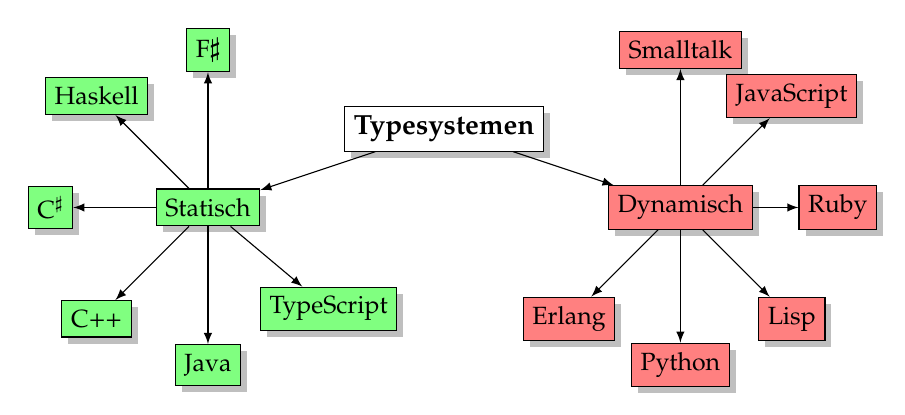
\begin{tikzpicture}[node/.style={drop shadow,draw,font=\small,fill=white},
                        static/.style={node,fill=green!50},
                        dynamic/.style={node,fill=red!50},
                        link/.style={-latex}]
      \node[node,font=\bfseries] (root) at (0,5) {Typesystemen};
      \visible<2->{
        \node[static] (static) at ($ (root) + (-3,-1) $) {Statisch};
        \node[dynamic] (dynamic) at ($ (root) + (3,-1) $) {Dynamisch};
        \draw[link] (root) -- (static);
        \draw[link] (root) -- (dynamic);
      }

      \visible<3->{
        \node[static] (java) at ($ (static) + (-90:2) $) {Java};
        \node[static] (cpp) at ($ (static) + (-135:2) $) {C++};
        \node[static] (csharp) at ($ (static) + (-180:2) $) {C$^\sharp$};
        \node[static] (haskell) at ($ (static) + (-225:2) $) {Haskell};
        \node[static] (typescript) at ($ (static) + (-40:2) $) {TypeScript};
        \node[static] (fsharp) at ($ (static) + (90:2) $) {F$\sharp$};

        \draw[link] (static) -- (java);
        \draw[link] (static) -- (cpp);
        \draw[link] (static) -- (csharp);
        \draw[link] (static) -- (haskell);
        \draw[link] (static) -- (typescript);
        \draw[link] (static) -- (fsharp);

        \node[dynamic] (smalltalk) at ($ (dynamic) + (90:2) $) {Smalltalk};
        \node[dynamic] (javascript) at ($ (dynamic) + (45:2) $) {JavaScript};
        \node[dynamic] (ruby) at ($ (dynamic) + (0:2) $) {Ruby};
        \node[dynamic] (lisp) at ($ (dynamic) + (-45:2) $) {Lisp};
        \node[dynamic] (python) at ($ (dynamic) + (-90:2) $) {Python};
        \node[dynamic] (erlang) at ($ (dynamic) + (-135:2) $) {Erlang};

        \draw[link] (dynamic) -- (smalltalk);
        \draw[link] (dynamic) -- (javascript);
        \draw[link] (dynamic) -- (ruby);
        \draw[link] (dynamic) -- (lisp);
        \draw[link] (dynamic) -- (python);
        \draw[link] (dynamic) -- (erlang);
      }
    \end{tikzpicture}
  \end{center}
\end{frame}

\subsection{Statisch Getypeerd}

\frame{\tableofcontents[currentsubsection]}

\begin{frame}
  \frametitle{Statisch Getypeerde Talen}
  \begin{itemize}
    \item Analyseren de code
    \item Weigeren te compileren bij typefouten
    \item Code moet meestal type-annotaties bevatten
  \end{itemize}
  \begin{center}
    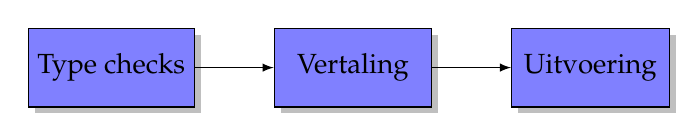
\begin{tikzpicture}[every node/.style={fill=blue!50,drop shadow,draw,minimum width=2cm,minimum height=1cm},link/.style={-latex}]
      \node (static analysis) at (0,0) {Type checks};
      \node[anchor=west] (compilation) at ($ (static analysis.east) + (1,0) $) {Vertaling};
      \node[anchor=west] (runtime) at ($ (compilation.east) + (1,0) $) {Uitvoering};

      \draw[link] (static analysis) -- (compilation);
      \draw[link] (compilation) -- (runtime);
    \end{tikzpicture}
  \end{center}
\end{frame}

\begin{frame}
  \frametitle{Voorbeeld}
  \code[language=java,width=.6\linewidth]{Min.java}
  \begin{tikzpicture}[remember picture,overlay,
                      message/.style={opacity=0.75,text opacity=1,fill=red!50,draw,drop shadow},
                      link/.style={-latex}]
    \only<2>{
      \codeunderlinex{return}
      \codeunderlinex{x type}
      \codeunderlinex{y type}
      \node[message] (type annotations) at ($ (x type) + (0,-1) $) {Type annotaties};
      \draw[link] (type annotations.north) -- (x type);
      \draw[link] (type annotations) -| (y type);
      \draw[link] (type annotations) -| (return);
    }

    \only<3>{
     \codeunderlinex{comparison}
      \node[message] (comparable) at ($ (comparison) + (2,-1) $) {Kunnen \texttt{x} en \texttt{y} vergeleken worden?};
      \draw[link] let \p1=(comparison), \p2=(comparable.north) in (\x1,\y2) -- (\p1);
    }

    \only<4>{
      \codeunderlinex{x type}
      \codeunderlinex{y type}
      \node[message] (comparable) at ($ (y type) + (0,-1) $) {Ja, het zijn beide \texttt{int}s};
      \draw[link] let \p1=(x type), \p2=(comparable.north) in (\x1,\y2) -- (\p1);
      \draw[link] let \p1=(y type), \p2=(comparable.north) in (\x1,\y2) -- (\p1);
    }

    \only<5>{
     \codeunderlinex{comparison}
      \node[message] (boolean) at ($ (comparison) + (2,-1) $) {\texttt{if} verwacht \texttt{boolean}, dit is ok};
      \draw[link] let \p1=(comparison), \p2=(boolean.north) in (\x1,\y2) -- (\p1);
    }

    \only<6>{
      \codeunderlinex{return x}
      \node[message] (returnable) at ($ (return x) + (2,-1) $) {Mag \texttt{x} gereturnd worden?};
      \draw[link] let \p1=(return x), \p2=(returnable.north) in (\x1,\y2) -- (\p1);
    }

    \only<7>{
      \codeunderlinex{return}
      \codeunderlinex{x type}
      \node[message] (returnable) at ($ (x type) + (0,-1) $) {Ja, type \texttt{x} en returntype komen overeen};
      \draw[link] let \p1=(return), \p2=(returnable.north) in (\x1,\y2) -- (\p1);
      \draw[link] let \p1=(x type), \p2=(returnable.north) in (\x1,\y2) -- (\p1);
    }

    \only<8>{
      \codeoverlinex{return y}
      \node[message] (returnable) at ($ (return y) + (2,1) $) {Mag \texttt{y} gereturnd worden?};
      \draw[link] let \p1=(return y), \p2=(returnable.south) in (\x1,\y2) -- (\p1);
    }

    \only<9>{
      \codeunderlinex{return}
      \codeunderlinex{y type}
      \node[message] (returnable) at ($ (x type) + (0,-1) $) {Ja, type \texttt{y} en returntype komen overeen};
      \draw[link] let \p1=(return), \p2=(returnable.north) in (\x1,\y2) -- (\p1);
      \draw[link] let \p1=(y type), \p2=(returnable.north) in (\x1,\y2) -- (\p1);
    }
  \end{tikzpicture}
\end{frame}

\begin{frame}
  \frametitle{Statische Typering}
  \structure{Voordelen}
  \begin{itemize}
    \item Fouten worden op voorhand gedetecteerd
    \item Leidt tot snellere code
    \item Garantie op ontbreken van typefouten
    \item H\'e\'el nuttig voor grote teams
  \end{itemize}
  \vskip5mm
  \structure{Nadelen}
  \begin{itemize}
    \item Legt strikte beperkingen op
    \item Leidt vaak tot veel boilerplate code
  \end{itemize}
\end{frame}

\subsection{Dynamisch Getypeerd}

\frame{\tableofcontents[currentsubsection]}

\begin{frame}
  \frametitle{Dynamisch Getypeerde Talen}
  \begin{itemize}
    \item Geen code analyse
    \item Tijdens uitvoering krijgen alle objecten een ``type tag''
    \item Type tag identificeert type
    \item Alle type checks gebeuren tijdens uitvoering
  \end{itemize}
  \begin{center}
    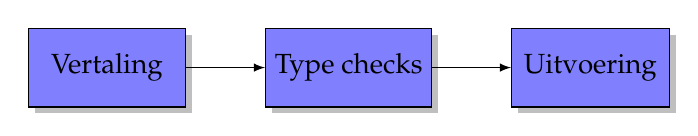
\begin{tikzpicture}[every node/.style={fill=blue!50,drop shadow,draw,minimum width=2cm,minimum height=1cm},link/.style={-latex}]
      \node (translation) at (0,0) {Vertaling};
      \node[anchor=west] (type checks) at ($ (translation.east) + (1,0) $) {Type checks};
      \node[anchor=west] (runtime) at ($ (type checks.east) + (1,0) $) {Uitvoering};

      \draw[link] (translation) -- (type checks);
      \draw[link] (type checks) -- (runtime);
    \end{tikzpicture}
  \end{center}
\end{frame}

\begin{frame}
  \frametitle{Dynamische Typering}
  \structure{Voordelen}
  \begin{itemize}
    \item Geeft veel meer vrijheid
    \item Code herbruikbaarder
    \item Kortere code
    \item Eenvoudiger te begrijpen
  \end{itemize}
  \vskip5mm
  \structure{Nadelen}
  \begin{itemize}
    \item Trager
    \item Fouten pas ontdekt tijdens uitvoering
    \item Afgeraden voor grote projecten
  \end{itemize}
\end{frame}

\subsection{Effici\"entie}

\frame{\tableofcontents[currentsubsection]}

\begin{frame}
  \frametitle{Statisch Getypeerde Talen}
  \code[language=java]{add.java}
  Vertaling:
  \code{add.asm}
\end{frame}

\begin{frame}
  \frametitle{Dynamisch Getypeerde Talen}
  \code[language=python]{add.py}
  Mogelijke vertaling (pseudoassembly):
  \code[font=\tiny,width=.4\linewidth]{add-dynamic.asm}
\end{frame}


%%% Local Variables:
%%% mode: latex
%%% TeX-master: "python"
%%% End:

\section{Praktische Informatie}

\frame{\tableofcontents[currentsection]}


\begin{frame}
  \frametitle{Python Versies}
  \begin{center}
    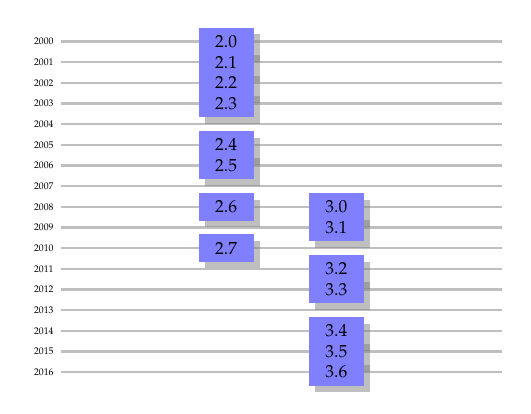
\begin{tikzpicture}[version/.style={drop shadow,fill=blue!50,minimum height=0.5cm,minimum width=1cm,font=\small},
                        timeline/.style={gray!50,thick},
                        scale=0.7,transform shape]
      \tikzmath{
        function yeary(\year) {
          return -(\year - 2000)*0.375;
        };
      }
      \foreach[count=\i,evaluate={yeary(\year)} as \y] \year in {2000,...,2016} {
        \draw[timeline] (0,\y) -- ++(8,0) node[at start,font=\tiny,left,black] {\year};
      }

      \foreach[count=\i] \version/\year in {2.0/2000,2.1/2001,2.2/2002,2.3/2003,2.4/2005,2.5/2006,2.6/2008,2.7/2010} {
        \tikzmath{
          real \y;
          \y = yeary(\year);
        }
        \node[version] at (3,\y) {\version};
      }

      \foreach[count=\i] \version/\year in {3.0/2008,3.1/2009,3.2/2011,3.3/2012,3.4/2014,3.5/2015,3.6/2016} {
        \tikzmath{
          real \y;
          \y = yeary(\year);
        }
        \node[version] at (5,\y) {\version};
      }
    \end{tikzpicture}
  \end{center}
  \begin{itemize}
    \item 3.0 voerde breaking changes in
    \item 2.x wordt nog in leven gehouden (legacy code)
    \item Dit vak: Python 3.5 (of beter)
  \end{itemize}
\end{frame}

\begin{frame}
  \frametitle{Benodigde Software}
  \begin{itemize}
    \item \link{https://www.python.org/downloads/release/python-360/}{Python 3.5 of beter}
    \item \link{https://git-scm.com/downloads}{Git}
          \begin{itemize}
            \item Windowsgebruikers: Git Bash!
          \end{itemize}
    \item Editor naar keuze
          \begin{itemize}
            \item \link{https://www.gnu.org/software/emacs/download.html}{Emacs} (voor de durvers)
            \item \link{https://vim.sourceforge.io/download.php}{VIM} (voor de masochisten)
            \item Notepad (voor de minimalisten)
            \item \link{https://notepad-plus-plus.org/}{Notepad++}
            \item \link{https://www.sublimetext.com/}{Sublime Text}
            \item Liefst niet MS Office
            \item \dots
          \end{itemize}
    \item Editor maakt weinig uit: we werken via command line
  \end{itemize}
\end{frame}

\begin{frame}
  \frametitle{Eerste Stappen}
  \begin{itemize}
    \item Cursusmateriaal staat op git repository
    \item Kies een locatie op je PC (bv. \texttt{c:\textbackslash git-repos})
          \begin{itemize}
            \item NIET onder Dropbox/OneDrive/\dots
          \end{itemize}
    \item Open Git Bash in deze directory
    \item Voer in (allemaal op \'e\'en lijn, \textvisiblespace\ staat voor spatie)
          \begin{center} \ttfamily\small
            git\textvisiblespace clone\textvisiblespace \\
            https://bitbucket.org/fvogels/ucll-scripting1617.git\textvisiblespace \\
            scripting
          \end{center}
          Of copy paste onderstaande lijn:
          \begin{center} \ttfamily\tiny
            git clone https://bitbucket.org/fvogels/ucll-scripting1617.git scripting
          \end{center}
    \item Enkel onder MacOS/Linux, in \texttt{scripts} subdirectory
          \begin{center} \ttfamily
            chmod u+x prepare run-tests show-help
          \end{center}
  \end{itemize}
\end{frame}

\begin{frame}
  \frametitle{Testen Configuratie}
  \begin{itemize}
    \item Python versie moet minimum 3.5 tonen
          \begin{center} \ttfamily
            python --version
          \end{center}
    \item Ga in repo-directory
          \begin{center} \ttfamily
            cd scripting
          \end{center}
    \item Ga naar de \texttt{scripts} subdirectory
          \begin{center} \ttfamily
            cd scripts
          \end{center}
    \item Voer in
          \begin{center} \ttfamily
            source setup
          \end{center}
    \item Ga naar \texttt{exercises/basics}
          \begin{center} \ttfamily
            cd ../exercises/basics
          \end{center}
    \item Run de tests
          \begin{center} \ttfamily
            rt
          \end{center}
  \end{itemize}
\end{frame}

\begin{frame}
  \frametitle{Algemeen Gebruik Cursusmateriaal}
  \begin{itemize}
    \item Altijd via Git Bash
    \item Altijd eerst \texttt{source setup} uitvoeren
          \begin{itemize}
            \item Instructies komen later over hoe dit te automatiseren
          \end{itemize}
    \item Tests runnen met \texttt{rt}
          \begin{itemize}
            \item Dit runt de tests in alle subdirectories
          \end{itemize}
    \item Oefeningen staan in directories onder \texttt{exercises}
    \item Oefeningen volgen zelfde patroon
          \begin{itemize}
            \item \texttt{tests.py} bevat de tests
            \item \texttt{solution.py} bevat de oplossingen
            \item \texttt{student.py} is het bestand waarin je zelf moet werken
            \item \texttt{readme.txt} bevat uitleg
          \end{itemize}
  \end{itemize}
\end{frame}

\begin{frame}
  \frametitle{Demo}
  \begin{itemize}
    \item Ga naar \texttt{exercises/basics/00-demo}
    \item Vraag om extra uitleg
          \begin{center} \ttfamily
            h
          \end{center}
    \item Run de tests
          \begin{center} \ttfamily
            rt
          \end{center}
    \item Bekijk de output
    \item Extra output te verkrijgen met \texttt{rt -c}
    \item Pas \texttt{student.py} aan
    \item Run de tests opnieuw
          \begin{center} \ttfamily
            rt
          \end{center}
  \end{itemize}
\end{frame}

\begin{frame}
  \frametitle{Algemene Aanpak}
  \begin{itemize}
    \item Veel online bronnen als hulp
    \item Suggestie: \link{http://tutorialspoint.com/python/}{tutorialspoint}
    \item Belangrijk om zelf dingen op te zoeken
    \item Vergeet ook niet om de dingen ook te begrijpen!
    \item Programmeren != kennen
    \item Programmeren = kunnen opzoeken, lezen, begrijpen
  \end{itemize}
\end{frame}


%%% Local Variables:
%%% mode: latex
%%% TeX-master: "python"
%%% End:





% Python specifieke stuff vs ...

\end{document}



%%% Local Variables: 
%%% mode: latex
%%% TeX-master: t
%%% End: 
